%
% 2-cauchyschwarz.tex
%
% (c) 2022 Prof Dr Andreas Müller, OST Ostschweizer Fachhochschule
%
\section{Ungleichungen
\label{buch:skalarprodukte:section:cauchyschwarz}}
\kopfrechts{Cauchy-Schwarz-Ungleichung}
%
% dreieck.tex
%
% (c) 2023 Prof Dr Andreas Müller
%
\begin{figure}
\centering
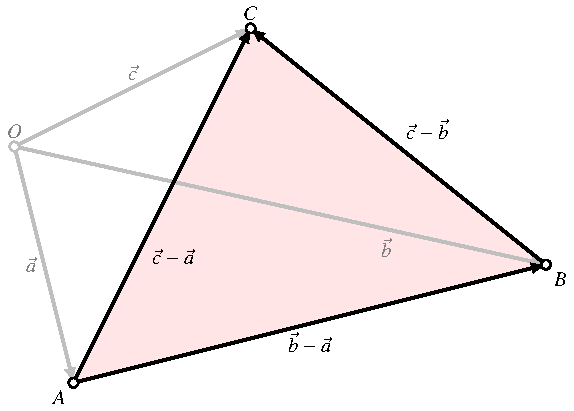
\includegraphics{chapters/010-skalarprodukt/images/dreieck.pdf}
\caption{Die Dreiecksungleichung ist gleichbedeutend mit der
Cauchy-Schwarz-Ungleichung.
\label{buch:skalarprodukt:ungleichungen:fig:dreieck}}
\end{figure}

In der Vektorgeometrie wird gelehrt, dass die Länge eines Vektors $u$
durch die Norm $\|u\|$ wiedergegeben wird.
Die geoemtrische Intuition der Länge, die sich in der Dreiecksungleichung
und dem Satz des Pythagoras äussert, ist auf die Norm anwendbar.
In anderen Räumen als dem dreidimensionalen Raum steht
jedoch keine geometrische Anschauung zur Verfügung, es muss also
auf anderen Wegen sichergestellt werden, dass die Intuition weiterhin
für das Rechnen mit dem Skalarprodukt und der zugehörigen Norm
funktioniert.
Dazu gehört vor allem, dass die Dreiecksungleichung erfüllt ist,
dass also für drei Punkt $A$, $B$ und $C$
\begin{equation}
\overline{AB} \le \overline{AC} + \overline{BC}
\label{skalarprodukt:ungleichungen:eqn:dreieck}
\end{equation}
gilt (Abbildung~\ref{buch:skalarprodukt:ungleichungen:fig:dreieck}).
In Vektorform bedeutet dies, dass
\[
\| b-a\|
\le
\| c-a\| + \|b-c\|.
\]
Schreibt man $u=c-a$ und $v=b-c$, dann ist $u+v=b-a$ und somit
\begin{equation}
\| u+v\| \le \|u\| + \|v\|.
\label{skalarprodukt:cauchyschwarz:eqn:dreieck0}
\end{equation}
Dies ist die Dreiecksungleichung in
Vektorform~\eqref{skalarprodukt:cauchyschwarz:eqn:dreieck0}.
Ziel dieses Abschnitts ist zu zeigen, dass jedes reelle oder
komplexe Skalarprodukt diese und weitere Eigenschaften automatisch
mitbringt.

%
% Cauchy-Schwarz-Ungleichung
%
\subsection{Cauchy-Schwarz-Ungleichung}
Sei also $\langle\;\,,\;\rangle$ ein reelles oder komplexes Skalarprodukt
auf dem Vektorraum $V$,
insbesondere ist $\langle v,v\rangle\ge 0$ für beliebige Vektoren $v\in V$.
Für zwei Vektoren $x,y\in V$ und $t\in \mathbb{R}$  gilt daher
\begin{align}
0
&\le
\| x+ty\|^2
=
\langle x+ty,x+ty\rangle
=
\langle x,x\rangle
+
t\langle x,y\rangle
+
t\langle y,x\rangle
+
t^2
\langle y,y\rangle.
\label{skalarprodukt:cauchyschwarz:eqn:quadrat}
\end{align}
Für ein reelles Skalarprodukt ist $\langle x,y\rangle=\langle y,x\rangle$
und damit
\begin{align}
0
&\le
\|x\|^2 + 2t\langle x,y\rangle + t^2 \|y\|^2.
\label{buch:skalarprodukt:cauchyschwarz:eqn:cspoly}
\end{align}
Dies ist ein quadratisches Polynom in der Variablen $t$, dessen Minimum
nicht negativ sein darf.

%
% Minimum eines quadratischen Polynoms
%
\subsubsection{Minimum eines quadratischen Polyoms}
Ein beliebiges quadratisches Polynom
\[
p(t)=at^2+bt+c
\]
kann durch
quadratisches Ergänzen in die Form
\[
p(t)
=
a\biggl(t+\frac{b}{2a}\biggr)^2 -\frac{b^2}{4a}+c
\]
gebracht werden.
Daraus kann man ablesen, dass das Minimum an der Stelle
\begin{equation}
t_0
=
-\frac{b}{2a}
\label{buch:skalarprodukt:definition:def:t0}
\end{equation}
angenommen wird und den Wert 
\begin{equation}
p(t_0)
=
c-\frac{b^2}{4a}
\end{equation}
hat.
Die gleiche Lösung kann natürlich auch durch Bestimmung des Minimums
von $p(t)$ mit Hilfe der Bedingung $p'(t_0)=0$ gefunden werden.

%
% Cauchy-Schwarz-Ungleichung für einen reellen Vektorraum
%
\subsubsection{Cauchy-Schwarz-Ungleichung für einen reellen Vektorraum}
Die rechte Seite von
\eqref{buch:skalarprodukt:cauchyschwarz:eqn:cspoly}
ist ein quadratisches Polynom mit den Koeffizienten
\[
a=\|y\|^2,\quad
b=2\langle x,y\rangle
\quad\text{und}\quad
c=\|x\|^2.
\]
Mit dem Wert
\[
t_0
=
-\frac{b}{2a}
=
-\frac{\langle x,y\rangle}{\|y\|^2}
\]
aus \eqref{buch:skalarprodukt:definition:def:t0} muss
\eqref{buch:skalarprodukt:cauchyschwarz:eqn:cspoly}
immer noch gelten, also
\[
0
\le
c-\frac{b^2}{2a}
=
\|x\|^2 - \frac{\langle x,y\rangle^2}{\|y\|^2}
\qquad\Rightarrow\qquad
\langle x,y\rangle^2 \le \|x\|^2\, \|y\|^2
\qquad\Rightarrow\qquad
|\langle x,y\rangle| \le \|x\|\cdot \|y\|.
\]
Dies ist die Cauchy-Schwarz-Ungleichung für das Skalarprodukt
$\langle \;\,,\;\rangle$.

\begin{satz}[Cauchy-Schwarz]
\label{buch:skalarprodukt:cauchy-schwarz:satz:reell}
Ein reelles Skalarprodukt $\langle\;\,,\;\rangle$ auf dem reellen Vektorraum
$V$ erfüllt die Cauchy-Schwarz-Ungleichung
\begin{equation}
|\langle x, y\rangle| \le \|x\|\cdot\|y\|
\label{buch:skalarprodukt:cauchyschwarz:eqn:ungleichung}
\end{equation}
für $x,y\in V$.
Gleichheit gilt genau dann, wenn $x$ und $y$ linear abhängig sind.
\end{satz}

\begin{proof}[Beweis]
Es ist nur noch die Aussage für die Gleichheit in der Ungleichung
\eqref{buch:skalarprodukt:cauchyschwarz:eqn:ungleichung}
zu beweisen.
Gleichheit kann nur eintreten, wenn nach
\eqref{skalarprodukt:cauchyschwarz:eqn:quadrat}
$x+ty=0$ wird.
Dies ist gleichbedeutend damit, dass $x$ und $y$ linear abhängig sind.
\end{proof}

%
% Cauchy-Schwarz-Ungleichung für einen komplexen Vektorraum
%
\subsubsection{Cauchy-Schwarz-Ungleichung für einen komplexen Vektorraum}
Für ein komplexes Skalarprodukt ist das Produkt $\langle x,y\rangle$
nicht mehr unbedingt reell und kann damit nicht mehr direkt mit den
Normen $\|x\|^2u$ und $\|y\|^2$ vergleichen.
Wir ersetzen daher $t$ durch
$t\langle y,x\rangle=t\overline{\langle x,y\rangle}$
und erhalten 
\begin{align*}
0
\le
\|x+t\langle y,x\rangle y\|^2
&=
\langle x,x\rangle
+t\langle y,x\rangle \langle x,y\rangle
+t\overline{\langle y,x\rangle}\langle y,x\rangle
+t^2\langle y,y\rangle
\\
&=
\|x\|^2
+
t
2|\langle x,y\rangle|^2
+
t^2 |\langle x,y\rangle|^2
\|y\|^2.
\end{align*}
Dies ist wieder ein quadratisches Polynom, diesmal mit den Koeffizienten
\[
a= |\langle x,y\rangle|^2 \|y\|^2,
\quad
b= 2|\langle x,y\rangle|^2
\quad\text{und}\quad
c= \|x\|^2.
\]
Das Minimum dieses Polynoms ist nach
\begin{align*}
0
&\le
c-\frac{b^2}{4a}
=
\|x\|^2 - \frac{|\langle x,y\rangle|^4}{|\langle x,y\rangle|^2\,\|y\|^2}
=
\|x\|^2 - \frac{|\langle x,y\rangle|^2}{\|y\|^2}
\\
\quad\Rightarrow\quad
|\langle x,y\rangle|^2 &\le \|x\|^2\,\|y\|^2
\\
\quad\Rightarrow\quad
|\langle x,y\rangle &\le \|x\|\cdot\|y\|.
\end{align*}
Dies ist die Cauchy-Schwarz-Ungleichung für einen komplexen Vektorraum.

\begin{satz}[Cauchy-Satz]
\label{buch:skalarprodukt:cauchy-schwarz:satz:komplex}
Ein komplexes Skalarprodukt $\langle\;\,,\;\rangle$ auf dem komplexen Vektorraum
$V$ erfüllt die Cauchy-Schwarz-Ungleichung
\[
|\langle x, y\rangle| \le \|x\|\cdot\|y\|
\]
für $x,y\in V$.
\end{satz}

Man beachte, dass die
Sätze~\ref{buch:skalarprodukt:cauchy-schwarz:satz:reell}
und
\ref{buch:skalarprodukt:cauchy-schwarz:satz:komplex}
nur die Axiome eines Skalarproduktes verwenden.
Sie gelten also
ganz unabhängig von der konkreten Definition des Skalarproduktes,
solange die Eigenschaften eines Skalarproduktes gegeben sind.
Diese Aussage macht keine Annahme darüber, wieviele linear unabhängige
Vektoren es in dem Vektorraum gibt, sie gilt daher
auch für unendlichdimensionale Vektorräume.

\begin{beispiel}
Die sesquilineare Funktion
\[
\langle x,y\rangle
=
\sum_{i=1}^n\overline{x}_i y_i
\]
für Vektoren $x,y\in\mathbb{C}^n$ ist positiv definit, denn
\[
\langle x,x\rangle
=
\sum_{i=1}^n \overline{x}_i x_i = \sum_{i=1}^n |x_i|^2 > 0
\]
für $x\ne 0$.
Nach Satz~\ref{buch:skalarprodukt:cauchy-schwarz:satz:komplex}
gilt daher
\[
\biggl|
\sum_{i=1}^n \overline{x}_i y_i
\biggr|
\le
\!\sqrt{\sum_{i=1}^n |x_i|^2}
\cdot
\!\sqrt{\sum_{i=1}^n |y_i|^2}
\quad\text{oder auch}\quad
\biggl|
\sum_{i=1}^n x_i y_i
\biggr|
\le
\!\sqrt{\sum_{i=1}^n |x_i|^2}
\cdot
\!\sqrt{\sum_{i=1}^n |y_i|^2}
\]
für beliebige Vektoren $x,y\in\mathbb{C}^n$.
\end{beispiel}

\begin{beispiel}
\label{buch:skalarprodukt:cauchyschwarz:beispiel:skalarprodukt}
Die sesquilineare Funktion
\[
\langle f,g\rangle
=
\int_a^b \overline{f(x)} g(x)\,dx
\]
für komplexwertige, stetige Funktion auf dem Intervall $[a,b]$
ist positiv definit, denn
\[
\langle f,f\rangle
=
\int_a^b \overline{f(x)} f(x)\,dx
=
\int_a^b |f(x)|^2\,dx
\ge 0
\]
für $f\ne 0$.
Nach Satz~\ref{buch:skalarprodukt:cauchy-schwarz:satz:komplex}
gilt daher
\begin{align*}
\biggl|\int_a^b \overline{f(x)}g(x)\,dx\biggr|
&\le
\!\sqrt{\int_a^b |f(x)|^2\,dx}
\cdot
\!\sqrt{\int_a^b |g(x)|^2\,dx}
\intertext{oder auch}
\biggl|\int_a^b f(x) g(x)\,dx\biggr|
&\le
\!\sqrt{\int_a^b |f(x)|^2\,dx}
\cdot
\!\sqrt{\int_a^b |g(x)|^2\,dx}
\end{align*}
für beliebige komplexwertige stetige Funktionen $f,g$ auf dem
Intervall $[a,b]$.
\end{beispiel}

%
% Dreiecksungleichung
%
\subsection{Dreiecksungleichung}
Die Intuition einer Längenmessung basiert auf der
Dreiecksungleichung~\eqref{skalarprodukt:ungleichungen:eqn:dreieck}.
Sie ist gleichbedeutend mit der
Vektorform~\eqref{skalarprodukt:cauchyschwarz:eqn:dreieck0}
der Ungleichung.

Die Cauchy-Schwarz-Ungleichung ermöglicht nun, diese Ungleichung
nachzurechnen.
Die Norm von $\|x+y\|^2$ ist
\[
\|x+y\|^2
=
\langle x+y,x+y\rangle
=
\langle x,x\rangle
+
\langle x,y\rangle
+
\langle y,x\rangle
+
\langle y,y\rangle
=
\|x\|^2 + 2\operatorname{Re}\langle x,y\rangle + \|y\|^2.
\]
Den mittleren Term kann man mit der Cauchy-Schwarz-Ungleichung
umformen:
\begin{align*}
\|x\|^2 + 2\operatorname{Re}\langle x,y\rangle + \|y\|^2.
&\le
\|x\|^2 + 2|\operatorname{Re}\langle x,y\rangle| + \|y\|^2.
\\
&\le
\|x\|^2 + 2|\langle x,y\rangle| + \|y\|^2.
\\
&\le
\|x\|^2 + 2\|x\|\,\|y\| + \|y\|^2
=
(\|x\| + \|y\|)^2.
\end{align*}
Durch Ziehen der Wurzel folgt
\[
\|x+y\| \le \|x\| + \|y\|.
\]
Damit ist der folgende Satz bewiesen.

\begin{satz}[Dreiecksungleichung]
Für die Norm zu einem beliebigen Skalarprodukt auf dem reellen
oder komplexen Vektorraum $V$ gilt die Dreiecksungleichung
\[
\|x+y\| \le \|x\| + \|y\|
\]
für $x,y\in V$.
\end{satz}

%
% Normen
%
\subsection{Normen
\label{skalarprodukt:cauchyschwarz:subsection:norm}}
Mit dem Skalarprodukt konnte die Norm eines Vektors definiert werden.
Mit diesem Längenbegriff wird es möglich auszudrücken, was es heissen
soll, dass eine Folge von Vektoren gegen einen Grenzwert konvergiert.
Das Skalarprodukt ist jedoch nicht die einzige Möglichkeit, eine 
Norm für den der Konstruktion eines Grenzwertbegriffs zu definieren.
Zum Beispiel kann man auf $\mathbb{C}^n$ die sogenannte $l^1$-Norm
definieren.

\begin{definition}
\label{buch:skalarprodukt:cauchyschwarz:def:l1}
Die Funktion
\[
\|x\|_1
=
\sum_{i=1}^n |x_i|
\]
für $x\in\mathbb{C}^n$ heisst die {\em $l^1$-Norm} auf $\mathbb{C}^n$.
\end{definition}

Die Funktion $\|\cdot\|_1$ ist eine Norm im Sinne der folgenden Definition.

\begin{definition}
\label{buch:skalarprodukt:cauchyschwarz:def:norm}
Eine Funktion $\normfunc \colon V\to\mathbb{R}$ auf einem reellen
oder komplexen Vektorraum $V$ heisst eine {\em Norm}, wenn Sie die
folgenden Bedingungen erfüllt
\begin{enumerate}
\item
$\|\lambda x\| = |\lambda|\, \|x\|$ für $x\in V$ und $\lambda\in \Bbbk$
\item
Für alle Vektoren $x\in V$ mit $x\ne 0$ gilt $\|x\|>0$.
\item
Dreiecksungleichung: $\|x+y\| \le \|x\| + \|y\|$ für alle $x,y\in V$
\end{enumerate}
\end{definition}

Es ist klar, dass die $l^1$-Norm die Bedingungen~1 und 2 erfüllt.
Aber auch die Bedingung~3 kann man leicht  nachprüfen:
\[
\|x+y\|_1
=
\sum_{i=1}^n |(x+y)_i|
=
\sum_{i=1}^n |x_i+y_i|
\le
\sum_{i=1}^n(|x_i|+|y_i|)
=
\sum_{i=1}^n|x_i|
+
\sum_{i=1}^n|y_i|
=
\|x\|_1 + \|y\|_1,
\]
wozu wir nur die Dreiecksungleichung $|a+b|\le |a| + |b|$ für reelle 
oder komplexe Zahlen $a,b$ benötigen.

\begin{beispiel}
Die Funktion
\[
x\mapsto \|x\|_\infty = \sup_{1\le i\le n} |x_i|
\]
ist eine Norm auf $\mathbb{C}^n$.

Auch in diesem Fall sind die Bedingungen~1 und 2 ganz offensichtlich erfüllt.
Für die Dreiecksungleichung rechnen
\begin{align*}
\|x+y\|_\infty
&=
\sup_{1\le i\le n} |x_i+y_i|
\le
\sup_{1\le i\le n} (|x_i|+|y_i|)
\le
\sup_{1\le i\le n} |x_i|+\sup_{1\le i\le n}|y_i|
=
\|x\|_\infty + \|y\|_\infty.
\end{align*}
Somit ist $\normfunc_\infty$ eine Norm auf $\mathbb{C}^n$.
\end{beispiel}

\begin{definition}
\label{buch:skalarprodukt:cauchyschwarz:def:supremum}
Die Norm
\begin{equation}
\|x\|_\infty = \sup_{1\le i\le n} |x_i|
\label{buch:skalarprodukt:cauchyschwarz:eqn:supremumnorm}
\end{equation}
heisst die {\em Supremum-Norm}.
\index{Supremum-Norm}
\end{definition}

%
% Polaridentität
%
\subsection{Polaridentität}
Die durch das Skalarprodukt definierte Norm
\( \|x\|^2=\langle x,x\rangle \)
ist nach Abschnitt~\ref{skalarprodukt:cauchyschwarz:subsection:norm}
ein Spezialfall einer Norm.
Ist es möglich, für eine Norm, die von einem Skalarprodukt herkommt,
das Skalarprodukt wieder zu rekonstruieren?

%
% Reelles Skalarprodukt aus der Norm
%
\subsubsection{Reelles Skalarprodukt aus der Norm}
Für ein reelles Skalarprodukt zeigt der folgende Satz, dass sich
das Skalarprodukt aus Werten der Norm rekonstruieren lässt.

\begin{satz}[Polaridentität]
\label{skalarprodukt:cauchyschwarz:satz:polarformel}
Ist $\|\cdot\|$ die Norm zu einem Skalarprodukt auf dem reellen Vektorraum
$V$, dann kann das Skalarprodukt zweier Vektoren $x,y\in V$ mittels
der sogenannten {\em Polaridentität}
\index{Polaridentität}%
\begin{equation}
\langle x, y\rangle
=
\frac12\bigl(
\|x+y\|^2 - \|x\|^2 - \|y\|^2 
\bigr)
\label{skalarprodukt:cauchyschwarz:eqn:polar}
\end{equation}
berechnet werden.
\end{satz}

\begin{proof}[Beweis]
Die Gleichung
\begin{align*}
\|x+y\|^2
&=
\langle x+y,x+y\rangle
=
\|x\|^2 + 2\langle x,y\rangle + \|y\|^2 
\end{align*}
kann nach $\langle x,y\rangle$ aufgelöst werden und ergibt
die behauptete Formel~\eqref{skalarprodukt:cauchyschwarz:eqn:polar}.
\end{proof}

% 
% Parallelogrammgleichung
%
\subsubsection{Parallelogrammgleichung}
\begin{figure}
\centering
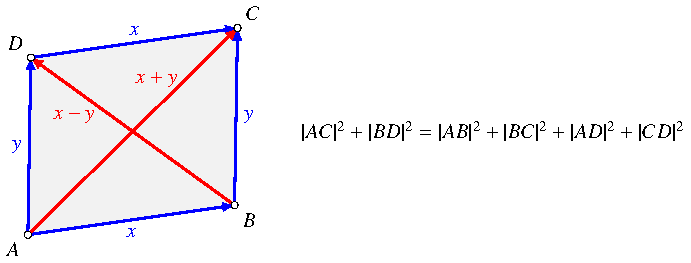
\includegraphics{chapters/010-skalarprodukt/images/parallelogramm.pdf}
\caption{Parallelogrammregel für eine Norm, die aus einem Skalarprodukt
entsteht.
\label{skalarprodukt:cauchyschwarz:fig:parallelogramm}}
\end{figure}
Die Polaridentitäten können auch noch in einer anderen Form geschrieben
werden.
Dazu berechnet man zusätzlich die Norm von $x-y$:
\begin{align*}
\|x+y\|^2
&=
\|x\|^2 + \|y\|^2 + 2\langle x, y\rangle
\\
\|x-y\|^2
&=
\|x\|^2 + \|y\|^2 - 2\langle x, y\rangle
\\
\|x+y\|^2 +\|x-y\|^2
&=
2\|x\|^2 + 2\|y\|^2
\end{align*}

\begin{satz}
\label{skalarprodukt:cauchyschwarz:satz:parallelgramm}
Für eine Norm, die von einem reellen Skalarprodukt herkommt, gilt die
Parallelogrammformel
\begin{equation}
\|x+y\|^2 +\|x-y\|^2
=
2\|x\|^2 + 2\|y\|^2.
\label{skalarprodukt:cauchyschwarz:eqn:parallelgramm}
\end{equation}
(Abbildung~\ref{skalarprodukt:cauchyschwarz:fig:parallelogramm})
\end{satz}

Das Skalarprodukt kann man damit auf verschiedene Weise aus der
Norm gewinnen:
\begin{equation}
\begin{aligned}
\langle x, y\rangle
&=
{\textstyle\frac12}\bigl( \|x\|^2 + \|y\|^2 - \|x+y\|^2 \bigr)
\\
&=
{\textstyle\frac12}\bigl(
\|x+y\|^2
-
\|x\|^2 
-
\|y\|^2
\bigr)
\\
&=
{\textstyle\frac14}\bigl(
\|x+y\|^2 - \|x-y\|^2
\bigr).
\end{aligned}
\label{skalarprodukt:cauchyschwarz:eqn:realteil}
\end{equation}
Nur die letzte Formel ist noch nicht gut begründet.
Man kann aber sofort nachrechnen, dass 
\begin{align*}
\|x+y\|^2&=\|x\|^2+2\langle x,y\rangle+\|y\|^2\\
\|x-y\|^2&=\|x\|^2-2\langle x,y\rangle+\|y\|^2
\intertext{die Differenz}
\|x+y\|^2 - \|x-y\|^2 &= 4\langle x,y\rangle
\qquad
\Rightarrow
\qquad
\langle x,y\rangle
=
\frac14\bigl(\|x+y\|^2 - \|x-y\|^2\bigr)
\end{align*}
haben.

%
% Komplexes Parallelogramm aus der Norm
%
\subsubsection{Komplexe Skalarprodukte}
Das Resultat von Satz~\ref{skalarprodukt:cauchyschwarz:satz:polarformel}
gilt in abgeänderter Form auch für komplexe Skalarprodukte.
Da das Skalarprodukt auch einen nichtverschwindenen Imaginärteil haben
kann, wird eine zusätzliche Gleichung zur Berechnung des Imaginärteils
nötig.
Eine solche kann gewonnen werden, indem zusätzlich die Normen
$\|x+iy\|^2$ und $\|x-iy\|^2$ berechnet werden.
Dazu ist zu beachten, dass
\[
\langle x,y\rangle
-
\langle y,x\rangle
=
\langle x,y\rangle
-
\overline{
\langle x,y\rangle
}
=
2i\operatorname{Im}\langle x,y\rangle
\]
Damit erhält man
\begin{align*}
\|x+iy\|^2 &= \|x\|^2 + i\langle x,y\rangle - i\langle y,x\rangle + \|y\|^2 
           = \|x\|^2 + 2\operatorname{Im}\langle x,y\rangle + \|y\|^2 \\
\|x-iy\|^2 &= \|x\|^2 - i\langle x,y\rangle + i\langle y,x\rangle + \|y\|^2 
           = \|x\|^2 - 2\operatorname{Im}\langle x,y\rangle + \|y\|^2.
\end{align*}
Damit kann man nach dem Imaginärteil des Skalarproduktes auflösen und
die Formeln
finden, die den Formeln
\eqref{skalarprodukt:cauchyschwarz:eqn:realteil}
für das reelle Skalarprodukt entsprechen.
Die Formeln
\eqref{skalarprodukt:cauchyschwarz:eqn:realteil}
bleiben gültig als Formeln für den Realteil des Skalarproduktes.
Damit haben wir den folgenden Satz gefunden.

\begin{satz}[Polaridentitäten für ein komplexes Skalarprodukt]
Ist $\|\cdot\|$ die Norm, die aus dem komplexen Skalarprodukt
$\langle\;\,,\;\rangle$ auf einem Vektorraum $V$ gewonnen wurde,
dann können Real- und Imaginärteil mit den Formeln
\begin{align*}
\operatorname{Re}\langle x,y\rangle
&=
{\textstyle\frac12}\bigl(
\|x+y\|^2 - \|x\|^2 -\|y\|^2
\bigr)
\\
&=
{\textstyle\frac12}\bigl(
\|x\|^2 +\|y\|^2 - \|x+y\|^2
\bigr)
\\
&=
{\textstyle\frac14}\bigl(
\|x+y\|^2 - \|x-y\|^2
\bigr),
\\
\operatorname{Im}\langle x,y\rangle
&=
{\textstyle\frac12}\bigl(
\|x+iy\|^2-\|x\|^2-\|y\|^2
\bigr)
\\
&=
{\textstyle\frac12}\bigl(
\|x\|^2+\|y\|^2-\|x-iy\|^2
\bigr)
\\
&=
{\textstyle\frac14}\bigl(
\|x+iy\|^2
-
\|x-iy\|^2
\bigr)
\end{align*}
für beliebige Vektoren $x,y\in V$
allein aus Werten der Norm berechnet werden.
\end{satz}

